% Problem 1

\Point{circuit_graph_and_circuit_001}{nodes}{1}
\Point{circuit_graph_and_circuit_001}{loops}{2}
\Point{circuit_graph_and_circuit_001}{branches}{1}
\Point{circuit_graph_and_circuit_001}{series}{1}
\Point{circuit_graph_and_circuit_001}{parallel}{1}
\Point{circuit_graph_and_circuit_001}{unknowns}{1}
\Point{circuit_graph_and_circuit_001}{kcl}{1}
\Point{circuit_graph_and_circuit_001}{kvl}{1}
\Point{circuit_graph_and_circuit_001}{ohm}{1}
\Point{circuit_graph_and_circuit_001}{solve}{13}
\begin{mainquestion}{circuit_graph_and_circuit_001}{Loops, Nodes, and Elements Oh My!}
Consider the following circuit diagram:

\begin{center}
    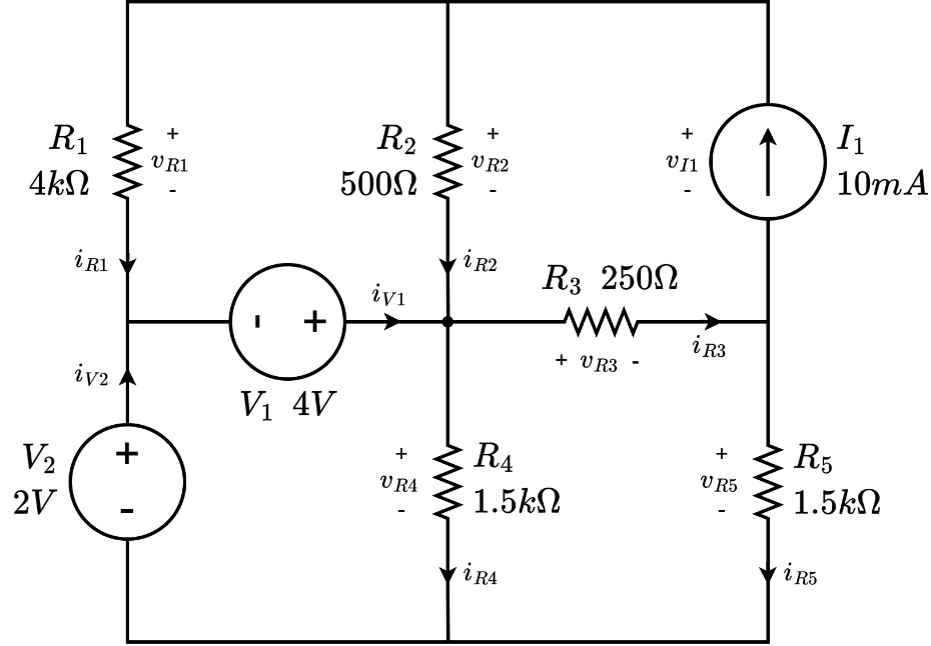
\includegraphics[]{questionbank/networks/circuit_graph/v1/schematic.png}
\end{center}

% =========================================================
\begin{partquestion}{nodes}
{How many nodes are in the circuit?}
\begin{answer}
    There are 5 nodes.
\end{answer}
\end{partquestion}

% =========================================================
\begin{partquestion}{loops}
{How many loops? How many independent loops?}
\begin{answer}
    There are 13 loops, although only 4 of them are independent.
\end{answer}
\end{partquestion}

% =========================================================
\begin{partquestion}{branches}
{How many branches?}
\begin{answer}
    There are 8 branches.  At this point, we can confirm the fundamental theorem of network topology:
    \begin{align*}
        b&=l+n-1\\
        &=4+5-1=8
    \end{align*}
\end{answer}
\end{partquestion}

% =========================================================
\begin{partquestion}{series}
{How many series elements are in the circuit?}
\begin{answer}
    There are no series elements in this circuit:  No two elements share a node exclusively.
\end{answer}
\end{partquestion}

% =========================================================
\begin{partquestion}{parallel}
{How many parallel elements are in the circuit?}
\begin{answer}
    There are no parallel elements in this circuit either!  No two elements share the same node at each of their respective terminals.
\end{answer}
\end{partquestion}
% =========================================================
\begin{partquestion}{unknowns}
{How many unknowns do you have?}
\begin{answer}
There are 7 unknown currents and 6 unknown voltages (don’t forget the voltage across the current source!).
\end{answer}
\end{partquestion}

% =========================================================
\begin{partquestion}{kcl}
{How many KCL equations?}
\begin{answer}
    There are 4 KCL equations (one for all but one node).
\end{answer}
\end{partquestion}

% =========================================================
\begin{partquestion}{kvl}
{How many KVL equations?}
\begin{answer}
There are 4 KVL equations (one for each independent loop).
\end{answer}
\end{partquestion}

% =========================================================
\begin{partquestion}{ohm}
{How many Ohm’s law equations?}
\begin{answer}
There are 5 Ohm’s law equations, one for each resistor.
\end{answer}
\end{partquestion}

% =========================================================
\begin{partquestion}{solve}
{Find all the unknown voltages (in \unit{\volt}) and currents (in \unit{\milli\ampere}) using systematic analysis of all equations found in (\cref{prob:circuit_graph_and_circuit_001:kcl}), (\cref{prob:circuit_graph_and_circuit_001:kvl}), and (\cref{prob:circuit_graph_and_circuit_001:ohm}).}

\begin{answer}

The four KCL equations are (here, current into a node is positive, and current out is negative):

\begin{align}
-i_{R1}-i_{R2}+\qty{10}{\milli\ampere} &= 0 \\
i_{R1}+i_{V2}-i_{V1} &= 0 \\
i_{V1}+i_{R2}-i_{R3}-i_{R4} &= 0 \\
i_{R3}-i_{R5}-\qty{10}{\milli\ampere} &= 0
\end{align}

The four KVL equations are (here the loops were taken in a counterclockwise fashion):

\begin{align}
\qty{4}{\volt}+\qty{2}{\volt}-v_{R4} &= 0 \\
-v_{R5}-v_{R3}+v_{R4} &= 0 \\
-v_{I1}+v_{R2}+v_{R3} &= 0 \\
-v_{R2}+v_{R1}-\qty{4}{\volt} &= 0
\end{align}

The five Ohm's law equations are:

\begin{align}
i_{R1} &= \frac{v_{R1}}{\qty{4}{\kilo\ohm}} \\
i_{R2} &= \frac{v_{R2}}{\qty{0.5}{\kilo\ohm}} \\
i_{R3} &= \frac{v_{R3}}{\qty{0.25}{\kilo\ohm}} \\
i_{R4} &= \frac{v_{R4}}{\qty{1.5}{\kilo\ohm}} \\
i_{R5} &= \frac{v_{R5}}{\qty{1.5}{\kilo\ohm}}
\end{align}

Here is one path to solving the circuit. Starting with (5), it is clear that
$v_{R4}=\qty{6}{\volt}$, and by equation (12)
$i_{R4}=\qty{4}{\milli\ampere}$. Now that $R_4$ is fully solved, equations (4) and (6) form a system of equations between $R_3$ and $R_5$. We substitute (11) and (13) into (4) and substitute $v_{R4}=\qty{6}{\volt}$ into equation (6). This leaves us with the following:
\begin{align*}
\frac{v_{R3}}{\qty{0.25}{\kilo\ohm}}
-
\frac{v_{R5}}{\qty{1.5}{\kilo\ohm}}
&=
\qty{10}{\milli\ampere} \\
v_{R3}+v_{R5}
&=
\qty{6}{\volt}
\end{align*}

Using the method of your choice to solve this system of equations, you will find
\begin{align*}
v_{R3} &= \qty{3}{\volt} \\
v_{R5} &= \qty{3}{\volt}
\end{align*}

Nice! Next use the Ohm's law relations for $R_3$ (11) and $R_5$ (13) to find
$i_{R3}=\qty{12}{\milli\ampere}$ and
$i_{R5}=\qty{2}{\milli\ampere}$.

We can repeat this technique using equations (1) and (8) as well as (9) and (10) to solve the voltages of $R_1$ and $R_2$. Here are the two equations after some massaging:

\begin{align*}
\frac{v_{R1}}{\qty{4}{\kilo\ohm}}
+
\frac{v_{R2}}{\qty{0.5}{\kilo\ohm}}
&=
\qty{10}{\milli\ampere} \\
v_{R1}-v_{R2}
&=
\qty{4}{\volt}
\end{align*}

Again, using the method of your choice to solve this system of equations, you will find

\begin{align*}
v_{R1} &= \qty{8}{\volt} \\
v_{R2} &= \qty{4}{\volt}
\end{align*}

Then plug back into (9) and (10) to find
$i_{R1}=\qty{2}{\milli\ampere}$ and
$i_{R2}=\qty{8}{\milli\ampere}$.

Now that we have all of the resistor branches and currents solved, we should easily be able to find the source unknowns from the remaining equations.

From equation (3) we see that

\[
i_{V1}
=
\qty{12}{\milli\ampere}
-
\qty{4}{\milli\ampere}
=
\qty{8}{\milli\ampere}.
\]

Plugging that into equation (2) reveals

\[
i_{V2}
=
\qty{8}{\milli\ampere}
-
\qty{2}{\milli\ampere}
=
\qty{6}{\milli\ampere}.
\]

Finally, equation (7) can be used to show

\[
v_{I1}
=
\qty{4}{\volt}
+
\qty{3}{\volt}
=
\qty{7}{\volt}.
\]

In summary, the determined values are captured in the tables below:

\begin{table}[htbp]
\centering

\begin{minipage}[t]{0.37\textwidth}
\centering
\begin{tabular}{|l|l|}
\hline
Unknown & Value \\ \hline
$v_{R1}$ & \qty{8}{\volt} \\ \hline
$v_{R2}$ & \qty{4}{\volt} \\ \hline
$v_{R3}$ & \qty{3}{\volt} \\ \hline
$v_{R4}$ & \qty{6}{\volt} \\ \hline
$v_{R5}$ & \qty{3}{\volt} \\ \hline
$v_{I1}$ & \qty{7}{\volt} \\ \hline
$i_{R1}$ & \qty{2}{\milli\ampere} \\ \hline
$i_{R2}$ & \qty{8}{\milli\ampere} \\ \hline
$i_{R3}$ & \qty{12}{\milli\ampere} \\ \hline
$i_{R4}$ & \qty{4}{\milli\ampere} \\ \hline
$i_{R5}$ & \qty{2}{\milli\ampere} \\ \hline
$i_{V1}$ & \qty{8}{\milli\ampere} \\ \hline
$i_{V2}$ & \qty{6}{\milli\ampere} \\ \hline
\end{tabular}
\end{minipage}
\hfill
\begin{minipage}[t]{0.60\textwidth}
\centering
\begin{tabular}{|l|c|c|l|}
\hline
Element & Voltage & Current & Power Flow \\ \hline
$R_1$ & \qty{8}{\volt} & \qty{2}{\milli\ampere} & Absorbing \\ \hline
$R_2$ & \qty{4}{\volt} & \qty{8}{\milli\ampere} & Absorbing \\ \hline
$R_3$ & \qty{3}{\volt} & \qty{12}{\milli\ampere} & Absorbing \\ \hline
$R_4$ & \qty{6}{\volt} & \qty{4}{\milli\ampere} & Absorbing \\ \hline
$R_5$ & \qty{3}{\volt} & \qty{2}{\milli\ampere} & Absorbing \\ \hline
V1 & \qty{4}{\volt} & \qty{8}{\milli\ampere} & Supplying \\ \hline
V2 & \qty{2}{\volt} & \qty{6}{\milli\ampere} & Supplying \\ \hline
I1 & \qty{7}{\volt} & \qty{10}{\milli\ampere} & Supplying \\ \hline
\end{tabular}
\end{minipage}

\end{table}

Note the current reference directions of the ideal sources do not obey the passive sign convention, so if you wanted to use the above table to analyze power you would have to insert negative signs on the currents for the three ideal sources. Adding up the powers for each element, we indeed verify that power is conserved
.
\[
P = 16 + 34 + 36 + 24 + 6 -32 - 12 - 70 = \qty{0}{\watt}
\]

\end{answer}
\end{partquestion}
\end{mainquestion}

% Problem 2
\clearpage
\Point{resistor_search}{findvalue}{10}
\Point{resistor_search}{deviation}{3}
\Point{resistor_search}{power}{3}
\begin{mainquestion}{resistor_search}{Resistor Ratios}

Consider a 220-mA current
source with source resistance $R_S$ connected to a
load $R_L$ as shown below. You
wish to find single, standard resistance values (1Ω
or higher) (assume \href{https://asenergi.com/pdf/resistors/standard-resistor-values-e24.pdf}{E24 series}—also in Hambley
Table B.1) for each resistor such that the current through the load is as close to 17 mA as possible, while minimizing the overall power dissipated in the circuit.

\begin{center}
    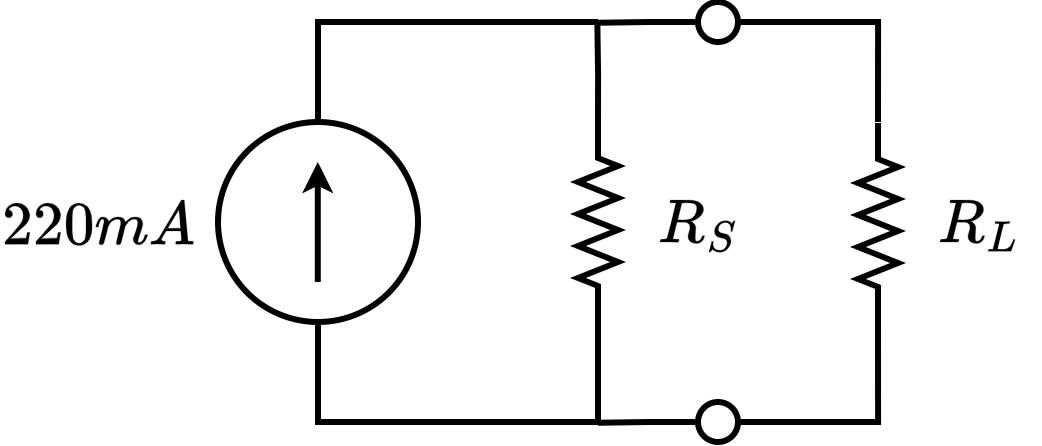
\includegraphics[width=0.5\textwidth]{questionbank/simple_circuits/resistor_search/v1/figure.png}
\end{center}

% =========================================================
\begin{partquestion}{findvalue}
{Find the values for $R_S$ and $R_L$ that satisfy these constraints, assuming the resistors accurately match their marked values.}

\begin{answer}
There are 24 standard resistance values within a decade of values; We only need consider one decade of values for the (smaller) $R_S$ since we will get identical results if we scale each resistor by a factor of ten:
\[
\frac{10R_S}{10R_S + 10R_L} = \frac{R_S}{R_S + R_L}
\]
Since the dissipated current will be of the form $P = I^2R$, we wish to make the resistances as small as possible to minimize this current dissipation, and we restrict our search to $\qty{1}{\ohm} \leq R_S \leq \qty{91}{\ohm}$. After choosing an $R_S$ we can find the optimal $R_L$ through the current divider relationship:
\begin{gather*}
I_L = \frac{R_S}{R_S + R_L}(I_{\text{source}}) \\
R_L = R_S(\frac{I_{\text{source}}}{I_L} - 1) = R_S(\frac{\qty{220}{\milli\ampere}}{\qty{17}{\milli\ampere}} - 1) = 11.941R_S
\end{gather*}
Then we can select an actual resistance value that is closest to $11.941R_S$ and record the deviation. Since this ratio is > 10 we know that $R_L$ must be one decade up. We can manually step through 24 calculations, or we can write a small script to find the best pair. The Python script below is not super-efficient because it looks at every pair of resistors and then sorts them, but it is simple to understand, and the speed of execution is not critical since the search space is so small.

\clearpage
\begin{lstlisting}
 Build the E24 series of resistors
E24 = [10, 11, 12, 13, 15, 16, 18, 20, 22, 24, 27, 30, 33, 36, 39, 43, 47, 51, 56, 62, 68, 75, 82, 91];
# Construct the E24 series of resistors shift down one decade
E24_down = [x / 10 for x in E24]

# Given a target current and load, find the best pair of resistors from the E24 series to achieve that ratio
supply = 0.22;
load = 0.017;
ratio = (supply / load) - 1;

# Build a list of all possible pairs of resistors from the E24 series and their ratios
results = []
for rs in E24_down:
    for rl in E24:
        pair = {
            'rs': rs,
            'rl': rl,
            'ratio': rl / rs
        }
        results.append(pair)

# Sort according to the absolute difference between the target ratio and the calculated ratio, and print the top 5 results
results.sort(key=lambda x: abs(x['ratio'] - ratio))
print("Target ratio: " + f"{ratio:.6f}")
for i in range(5):
    print(str(i + 1) + ": " + str(results[i]['rs']) + " and " + str(results[i]['rl']) + " with ratio " + f"{results[i]['ratio']:.6f}")
\end{lstlisting}

Executing this gives the following output:

\begin{lstlisting}
Target ratio: 11.941176
1: 3.6 and 43 with ratio 11.944444
2: 4.7 and 56 with ratio 11.914894
3: 1.0 and 12 with ratio 12.000000
4: 1.5 and 18 with ratio 12.000000
5: 2.0 and 24 with ratio 12.000000
\end{lstlisting}
So we have $R_S = \qty{3.6}{\ohm}$ and $R_L = \qty{43}{\ohm}$
\end{answer}
\end{partquestion}

% =========================================================
\begin{partquestion}{deviation}
{Calculate the \% deviation from the desired load current}

\begin{answer}
The two resistors above provide a load current of
\[I_L=\frac{\qty{3.6}{\ohm}}{\qty{3.6}{\ohm} + \qty{43}{\ohm}}(\qty{220}{\milli\ampere}) = \qty{16.996}{\milli\ampere}\]
which is a deviation of only
\[\frac{16.996-17}{17}\times100\% \approx0.025\%\]
\end{answer}
\end{partquestion}

% =========================================================
\begin{partquestion}{power}
{Calculate the total power dissipated in the circuit}

\begin{answer}
The total power dissipation is the sum of the power dissipated in each resistor. The current through the source resistor must be $220 - 16.996 = \qty{203.004}{\milli\ampere}$ and we can calculate
\[
P_{\text{total}} = P_{R_s} + P_{R_L} = {I_{R_S}}^2 R_S +{I_{R_L}}^2 R_L = (\qty{0.203}{\ampere})^2(\qty{3.6}{\ohm})+\qty{0.017}{\ampere}^2(\qty{43}{\ohm}) = \qty{0.16}{\watt}
\]
\end{answer}
\end{partquestion}

\end{mainquestion}

% Problem 3 function generators and oscilloscope probes
\clearpage
\Point{function_generator_and_scope}{mag}{2}
\Point{function_generator_and_scope}{power}{2}
\Point{function_generator_and_scope}{mag2}{2}
\Point{function_generator_and_scope}{voltadj}{2}
\Point{function_generator_and_scope}{power2}{2}
\Point{function_generator_and_scope}{sourcer}{2}
\Point{function_generator_and_scope}{secondscope}{2}
\begin{mainquestion}{function_generator_and_scope}{Function Generators and Oscilloscope Probes} As you may have seen in Lab 1, the function generators in the
laboratory can be simply configured with an output magnitude $V_m$.  Internally, this value is used to model a voltage source with amplitude $V_{\mathrm{gen}}$ which is placed in series with a $\qty{50}{\ohm}$ source resistance; this is illustrated in the accompanying circuit diagram.
By default, the function generator ``assumes'' it will be connected to a matched load; that is, a load $R_L$ whose resistance matches that of the source---namely
$\qty{50}{\ohm}$.


\begin{center}
    \includegraphics[width=4.7in]{circuit.png}
\end{center}

\begin{partquestion}{mag}{In a matched-load scenario, if the output (load) voltage is configured to have an amplitude of $\qty{10}{\volt}$, what is the actual value of $V_\mathrm{gen}$ set by the function generator?}
\begin{answer}
Because the function generator is expecting a matching load of $\qty{50}{\ohm}$, it expects
to deliver what is configured, $\qty{10}{\volt}$, at the load. Since
\[
V_L = V_{\mathrm{gen}}\frac{R_L}{\qty{50}{\ohm} + R_L},
\]
we have
\[
V_{\mathrm{gen}}
=V_L\frac{\qty{50}{\ohm}+R_L}{R_L}
=(\qty{10}{\volt})\frac{\qty{50}{\ohm}+\qty{50}{\ohm}}{\qty{50}{\ohm}}
=\qty{20}{\volt}.
\]
\end{answer}
\end{partquestion}
\begin{partquestion}{power}{What percentage of the power in the circuit is dissipated in the load in this scenario?}
\begin{answer}
For a periodic signal with amplitude $V_m$, the power dissipated in a resistor is always proportional to $\frac{V_m^2}{R_L}$.  
\[
P_L=\alpha\frac{V_L^2}{R_L}
=\alpha\frac{(\qty{10}{\volt})^2}{\qty{50}{\ohm}}
=2\alpha\,\mathrm{W}.
\]
The total power dissipated is
\[
P_{\mathrm{total}}
=\alpha\frac{V_{\mathrm{gen}}^2}{\qty{50}{\ohm}+R_L}
=\alpha\frac{(\qty{20}{\volt})^2}{\qty{100}{\ohm}}
=4\alpha\,\mathrm{W},
\]
so the percentage dissipated in the load is
\[
\frac{P_L}{P_{\mathrm{total}}}
=\frac{2\alpha\,\mathrm{W}}{4\alpha\,\mathrm{W}}
=0.5=50\%.
\]
\end{answer}
\end{partquestion}
\begin{partquestion}{mag2}{Now assume the load $R_L$ is not $\qty{50}{\ohm}$ but a $1\,\mathrm{M}\Omega$ oscilloscope channel input. If the function generator remains configured as in part (\cref{prob:function_generator_and_scope:mag}), what is the amplitude of the voltage that will be displayed on the oscilloscope?}
\begin{answer}
The internally generated source voltage remains $V_{\mathrm{gen}}=\qty{20}{\volt}$, but now
\[
V_L
=V_{\mathrm{gen}}\frac{1\,\mathrm{M}\Omega}
{\qty{50}{\ohm}+1\,\mathrm{M}\Omega}
\approx V_{\mathrm{gen}}
=\qty{20}{\volt}.
\]
\end{answer}
\end{partquestion}
\begin{partquestion}{voltadj}{How should the function-generator voltage be adjusted to provide the expected voltage across the load?}
\begin{answer}
We would need to drop the function-generator setting such that $V_m = \qty{5}{\volt}$, requiring that
\[
V_{\mathrm{gen}}=V_L=\qty{10}{\volt}.
\]
\end{answer}
\end{partquestion}
\begin{partquestion}{power2}{What percentage of the power in the circuit is now dissipated in the load?}
\begin{answer}
The power dissipated in the load is
\[
P_L=\alpha\frac{V_L^2}{R_L}
=\alpha\frac{(\qty{10}{\volt})^2}{1\,\mathrm{M}\Omega}
=0.1\alpha\,\mathrm{mW}.
\]
The total power dissipated is
\[
P_{\mathrm{total}}
=\alpha\frac{V_{\mathrm{gen}}^2}{\qty{50}{\ohm}+R_L}
=\alpha\frac{(\qty{10}{\volt})^2}{\qty{50}{\ohm}+1\,\mathrm{M}\Omega}
\approx 0.1\alpha\,\mathrm{mW},
\]
so the percentage dissipated in the load is approximately
\[
\frac{0.1\alpha\,\mathrm{mW}}{0.1\alpha\,\mathrm{mW}}
=1.0=100\%.
\]
\end{answer}
\end{partquestion}
\begin{partquestion}{sourcer}{What is the approximate source resistance of a $20{:}1$
oscilloscope probe?}
\begin{answer}
We require the voltage provided to the oscilloscope to be $1/20$ of the actual measured
voltage:
\[
\frac{V_{\mathrm{scope}}}{V_{\mathrm{probe}}}
=\frac{R_{\mathrm{scope}}}{R_{\mathrm{probe}}+R_{\mathrm{scope}}}
=\frac{1}{20}.
\]
Since the oscilloscope has a $1\,\mathrm{M}\Omega$ input,
\[
\frac{1\,\mathrm{M}\Omega}{R_{\mathrm{probe}}+1\,\mathrm{M}\Omega}
=\frac{1}{20},
\]
and therefore
\[
R_{\mathrm{probe}}=19\,\mathrm{M}\Omega.
\]
\end{answer}
\end{partquestion}
\begin{partquestion}{secondscope}{Now imagine you took such a probe attached (and properly configured)
to a second identical oscilloscope and measured the voltage of the load $R_L$ coming into
the first oscilloscope still configured as in part (\cref{prob:function_generator_and_scope:voltadj}). What is the voltage level seen by
the second oscilloscope? What is the voltage level displayed by the second oscilloscope?}
\begin{answer}
The voltage seen by the second oscilloscope is $1/20$ of the actual voltage, which was
determined to be $\qty{10}{\volt}$. Thus,
\[
V_{\mathrm{seen}}=\qty{0.5}{\volt}.
\]
Because the second oscilloscope is properly configured with the $20{:}1$ probe attenuation
factor, it compensates for this factor of 20 and displays
\[
V_{\mathrm{displayed}}=\qty{10}{\volt}.
\]
\end{answer}
\end{partquestion}

\end{mainquestion}




% Problem 4
\clearpage
\Point{wye_delta_nodal_no_dependent_source}{delta}{6}
\Point{wye_delta_nodal_no_dependent_source}{solve}{9}
\Point{wye_delta_nodal_no_dependent_source}{findvx}{2}
\Point{wye_delta_nodal_no_dependent_source}{deltakcl}{2}
\Point{wye_delta_nodal_no_dependent_source}{vcom}{2}
\Point{wye_delta_nodal_no_dependent_source}{wyekcl}{2}
\begin{mainquestion}{wye_delta_nodal_no_dependent_source}{Nodal Analysis + Delta/Wye}
Consider the following circuit. Note the top three resistors form a wye resistor network.

\begin{center}
    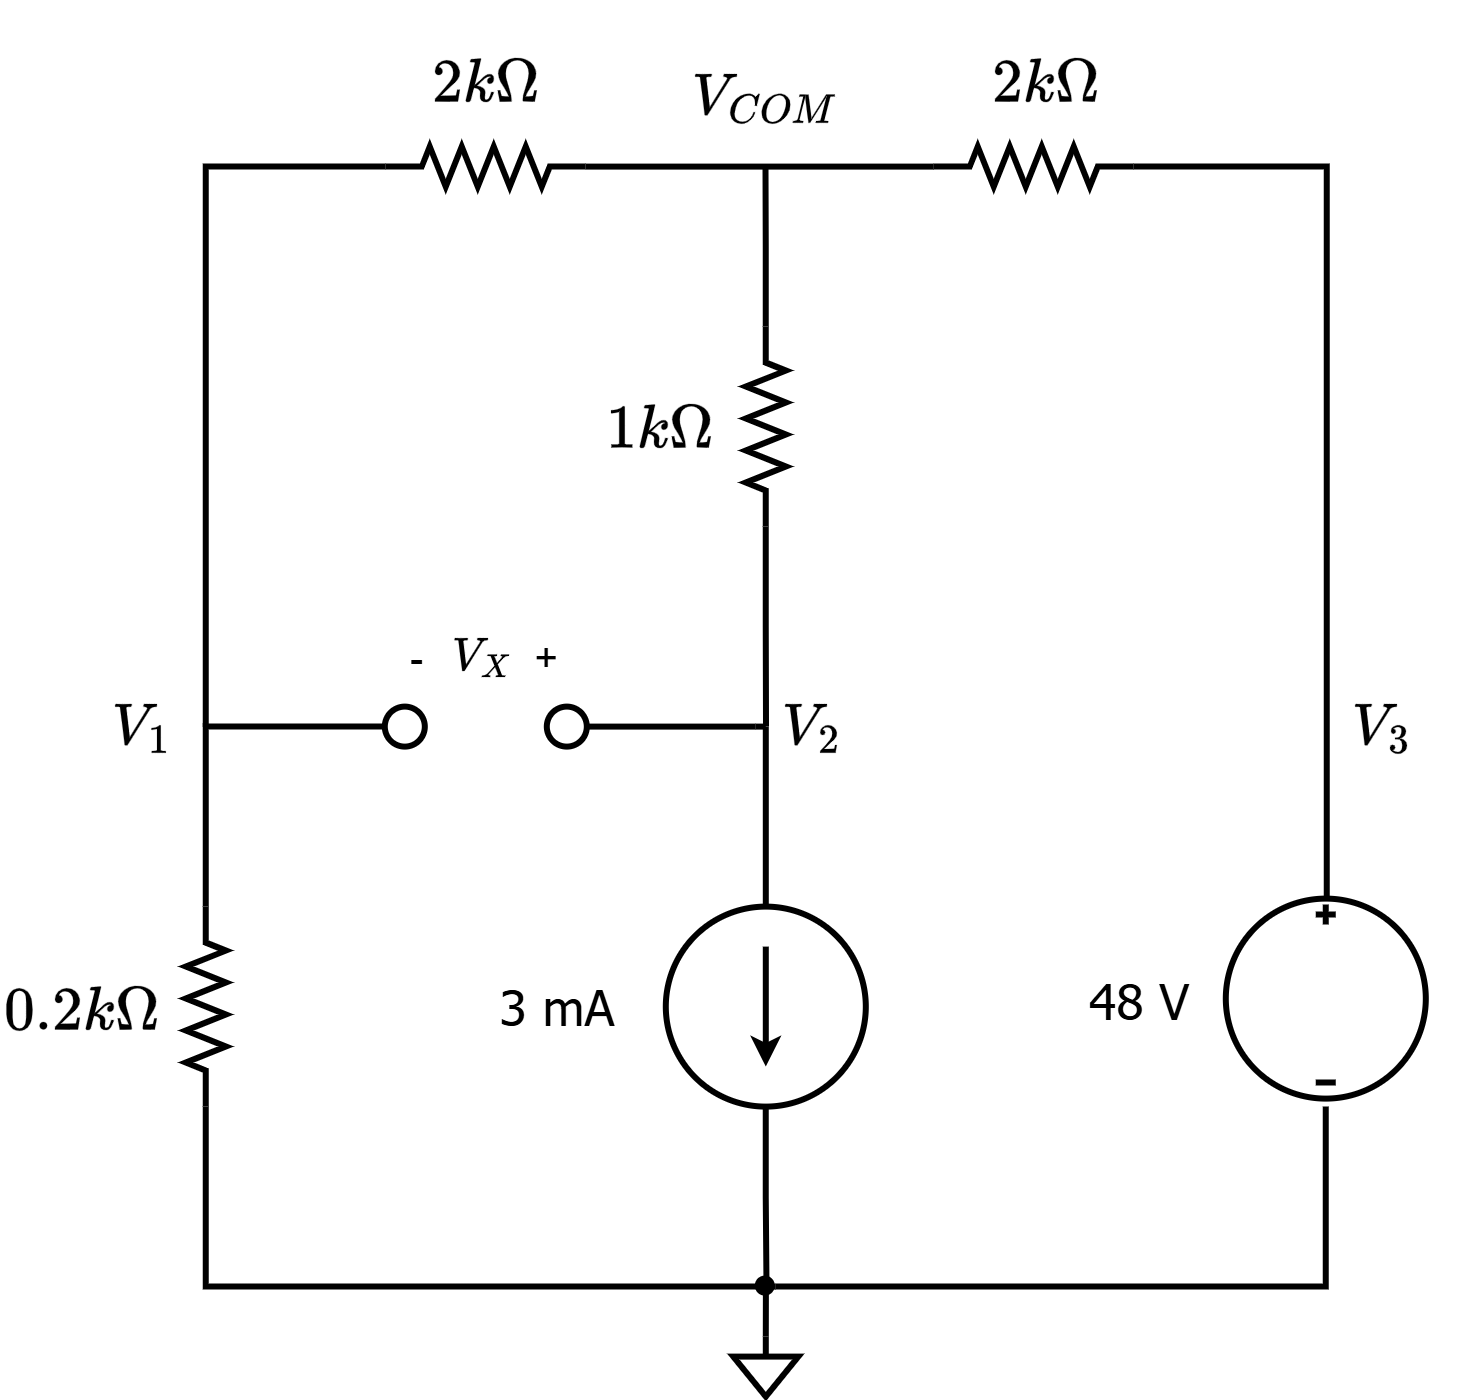
\includegraphics[width=0.6\textwidth]{questionbank/networks/wye_delta_nodal_no_dependent_source/v0/wye_sch.png}
\end{center}

% =========================================================
\begin{partquestion}{delta}
{Convert the wye network to a delta network with a Wye-Delta transform and redraw
the schematic. How many nodes exist in this equivalent circuit? How many nodes were
in the original?}
\begin{answer}
Looking at the Wye $\rightarrow$ Delta formulas, all of them use the same sum of the product pairs in their numerators. Let’s calculate that figure and we’ll call it $R_T$.
\[R_T=\ R_1R_2+R_2R_3+R_3R_1=4+2+2=\qty{8}{\mega\ohm}\]
Now we can calculate all the individual resistors. For the resistance between nodes $V_1$ and $V_2$, the equation will be $R_T/\qty{2}{\kilo\ohm} = \qty{4}{\kilo\ohm}$. For $V_2$ and $V_3$ we also have $R_T/\qty{2}{\kilo\ohm} = \qty{4}{\kilo\ohm}$ the odd one out will be the resistance between $V_1$ and $V_3$ which will be $R_T/\qty{1}{\kilo\ohm} = \qty{8}{\kilo\ohm}$. Here is the schematic with the new resistance values:

\begin{center}
    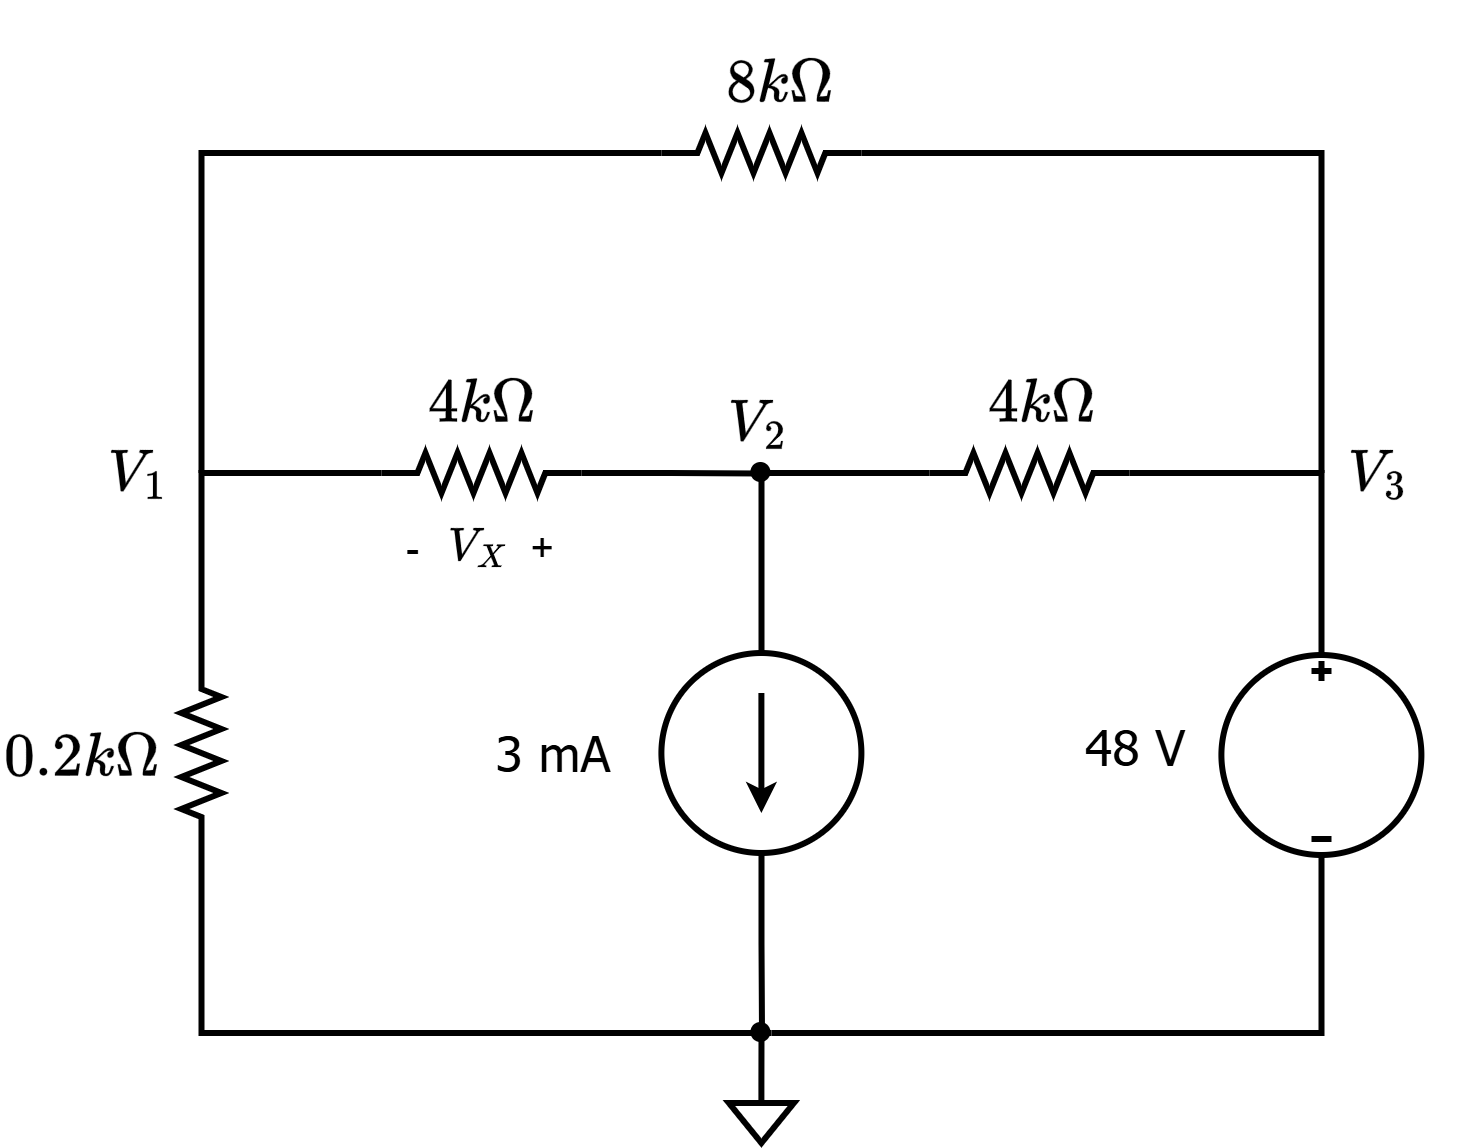
\includegraphics[width=0.5\textwidth]{questionbank/networks/wye_delta_nodal_no_dependent_source/v0/delta_sch_sol.png}
\end{center}

This new schematic has 4 nodes total, with only 3 independent nodes that require KCL equations. The original schematic had 5 nodes, with 4 independent nodes that need KCL equations. The transform effectively dropped one node for us.

\end{answer}
\end{partquestion}

% =========================================================
\begin{partquestion}{solve}
{Use nodal analysis on your new schematic to find each of the node voltages $V_1$, $V_2$ and $V_3$.}
\begin{answer}
We can leave out units, assuming all currents are \si{\milli\ampere}, all resistances are \si{\kilo\ohm}, and all voltages are \si{\volt}. Writing KCL using the nodal voltages at node 1 gives:
\begin{align*}
\frac{V_1}{0.2}+\frac{V_1-V_2}{4}+\frac{V_1-V_3}{8}&=0 \\
5V_1+\frac{V_1-V_2}{4}+\frac{V_1-V_3}{8}&=0 \\
40V_1+2(V_1-V_2)+(V_1-V_3)&=0 \\
43V_1-2V_2-V_3&=0
\end{align*}

Writing KCL using the nodal voltages at node 2 gives:
\begin{align*}
\frac{V_2-V_1}{4}+\frac{V_2-V_3}{4}+3&=0 \\
2V_2 - V_1 - V_3 &= -12
\end{align*}

We can see directly that $V_3 = 48$, so we can substitute this value into the two KCL equations above to get:
\begin{align*}
43V_1 - 2V_2 - 48&=0 \\
43V_1 - 2V_2 &= 48
\end{align*}
and
\begin{align*}
2V_2 - V_1 - 48 &= -12 \\
2V_2 - V_1 &= 36
\end{align*}

This gives two equations and two unknowns. Using your favorite method to solve systems of equations, we simply add the equations together to solve for the voltage at node 1:
\begin{align*}
43V_1 - V_1 &= 48 + 36 \\
42V_1 &= 84 \\
V_1 &= \qty{2}{\volt}
\end{align*}

Next we use this result with equation 2 to solve for the voltage at node 2:
\begin{align*}
2V_2 - 2 &= 36 \\
V_2 &= \frac{-38}{2} = \qty{19}{\volt}
\end{align*}

\end{answer}
\end{partquestion}

% =========================================================
\begin{partquestion}{findvx}
{Find $V_X$.}
\begin{answer}
\[V_X=V_2-V_1=19-2=\qty{17}{V}\]
Gotcha :)
\end{answer}
\end{partquestion}

% =========================================================
\begin{partquestion}{deltakcl}
{Given your results for $V_1$, $V_2$ and $V_3$, calculate all the branch currents in your new schematic. Show KCL is satisfied at each node.}

\begin{answer}
\begin{center}
    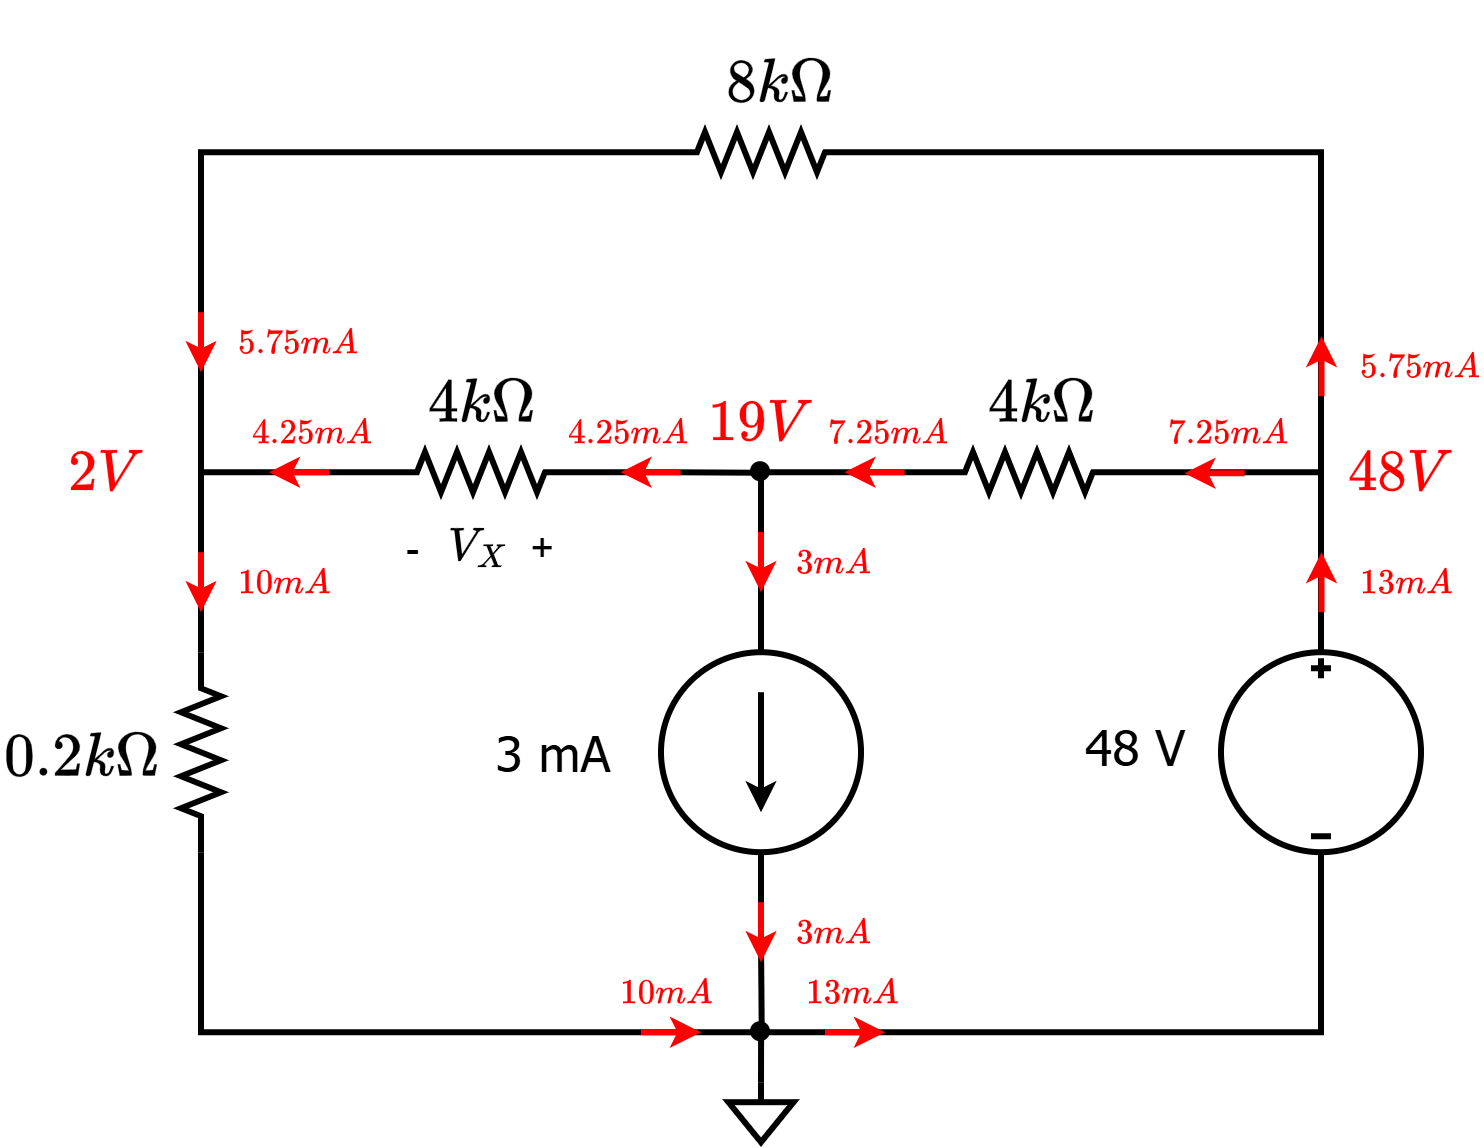
\includegraphics[width=0.5\textwidth]{questionbank/networks/wye_delta_nodal_no_dependent_source/v0/delta_kcl_sol.png}
\end{center}

Calculating the branch currents only requires Ohm’s Law for most of the branches. For example, the current through the top \qty{8}{\kilo\ohm} resistor is
\( I = \frac{V}{R} = \frac{\qty{48}{\volt} - \qty{2}{\volt}}{\qty{8}{\kilo\ohm}} = \qty{5.75}{\milli\ampere} \) and the current through the rightmost \qty{4}{\kilo\ohm} resistor is \( I = \frac{V}{R} = \frac{\qty{48}{\volt} - \qty{19}{\volt}}{\qty{4}{\kilo\ohm}} = \qty{7.25}{\milli\ampere} \). In a resistor, passive sign convention tells us that positive current flows in the direction of the voltage drop, so from left to right in this case. This can be repeated for the other resistors quite easily now that we have all of the voltage values. The only current that requires additional thought is the current through the dependent current source, which can be solved from the KCL equation at node 3.

\[
I_{48} = I_{8k\Omega} + I_{4k\Omega} = \qty{5.75}{\milli\ampere} + \qty{7.25}{\milli\ampere} = \qty{13}{\milli\ampere}
\]

Now we check that KCL is satisfied everywhere. There are 4 nodes where KCL needs to hold in this schematic. We’ll use positive values for currents flowing into a node:

At Node 1: \( 5.75 + 4.25 - 10 = 0 \)

At Node 2: \( 7.25 - 4.25 - 3 = 0 \)

At Node 3: \( 13 - 5.75 - 7.25 = 0 \)

At Ground: \( 10 + 3 - 13 = 0 \)

Look at that! All copacetic. We are now confident our solution is correct.

\end{answer}
\end{partquestion}

% =========================================================
\begin{partquestion}{vcom}
{Returning to the original schematic, find the voltage $V_{\text{COM}}$ given your results for $V_1$, $V_2$ and $V_3$.}
\begin{answer}
This is not too hard since we know the current in the \qty{1}{\kilo\ohm} resistor because it’s in series with the \qty{3}{\milli\ampere} current source. Thanks to Ohm’s Law, we know that there must be a \qty{3}{\volt} drop across it. Passive sign convention tells us that the voltage is highest on the side the current is coming from, so that implies that $V_{\mathrm{COM}}$ is \qty{3}{\volt} higher than $V_2$.

\[
V_{\mathrm{COM}} = V_2 + 3 = 19 + 3 = \qty{22}{\volt}
\]

This could also be solved with similar math using the right (\qty{13}{\milli\ampere}) or left (\qty{10}{\milli\ampere}) branches, as we already know that currents flowing through them from part (\cref{prob:wye_delta_nodal_no_dependent_source:deltakcl}).

\end{answer}
\end{partquestion}

% =========================================================
\begin{partquestion}{wyekcl}
{Repeat part (\cref{prob:wye_delta_nodal_no_dependent_source:deltakcl}) for the original schematic.}
\begin{answer}
\begin{center}
    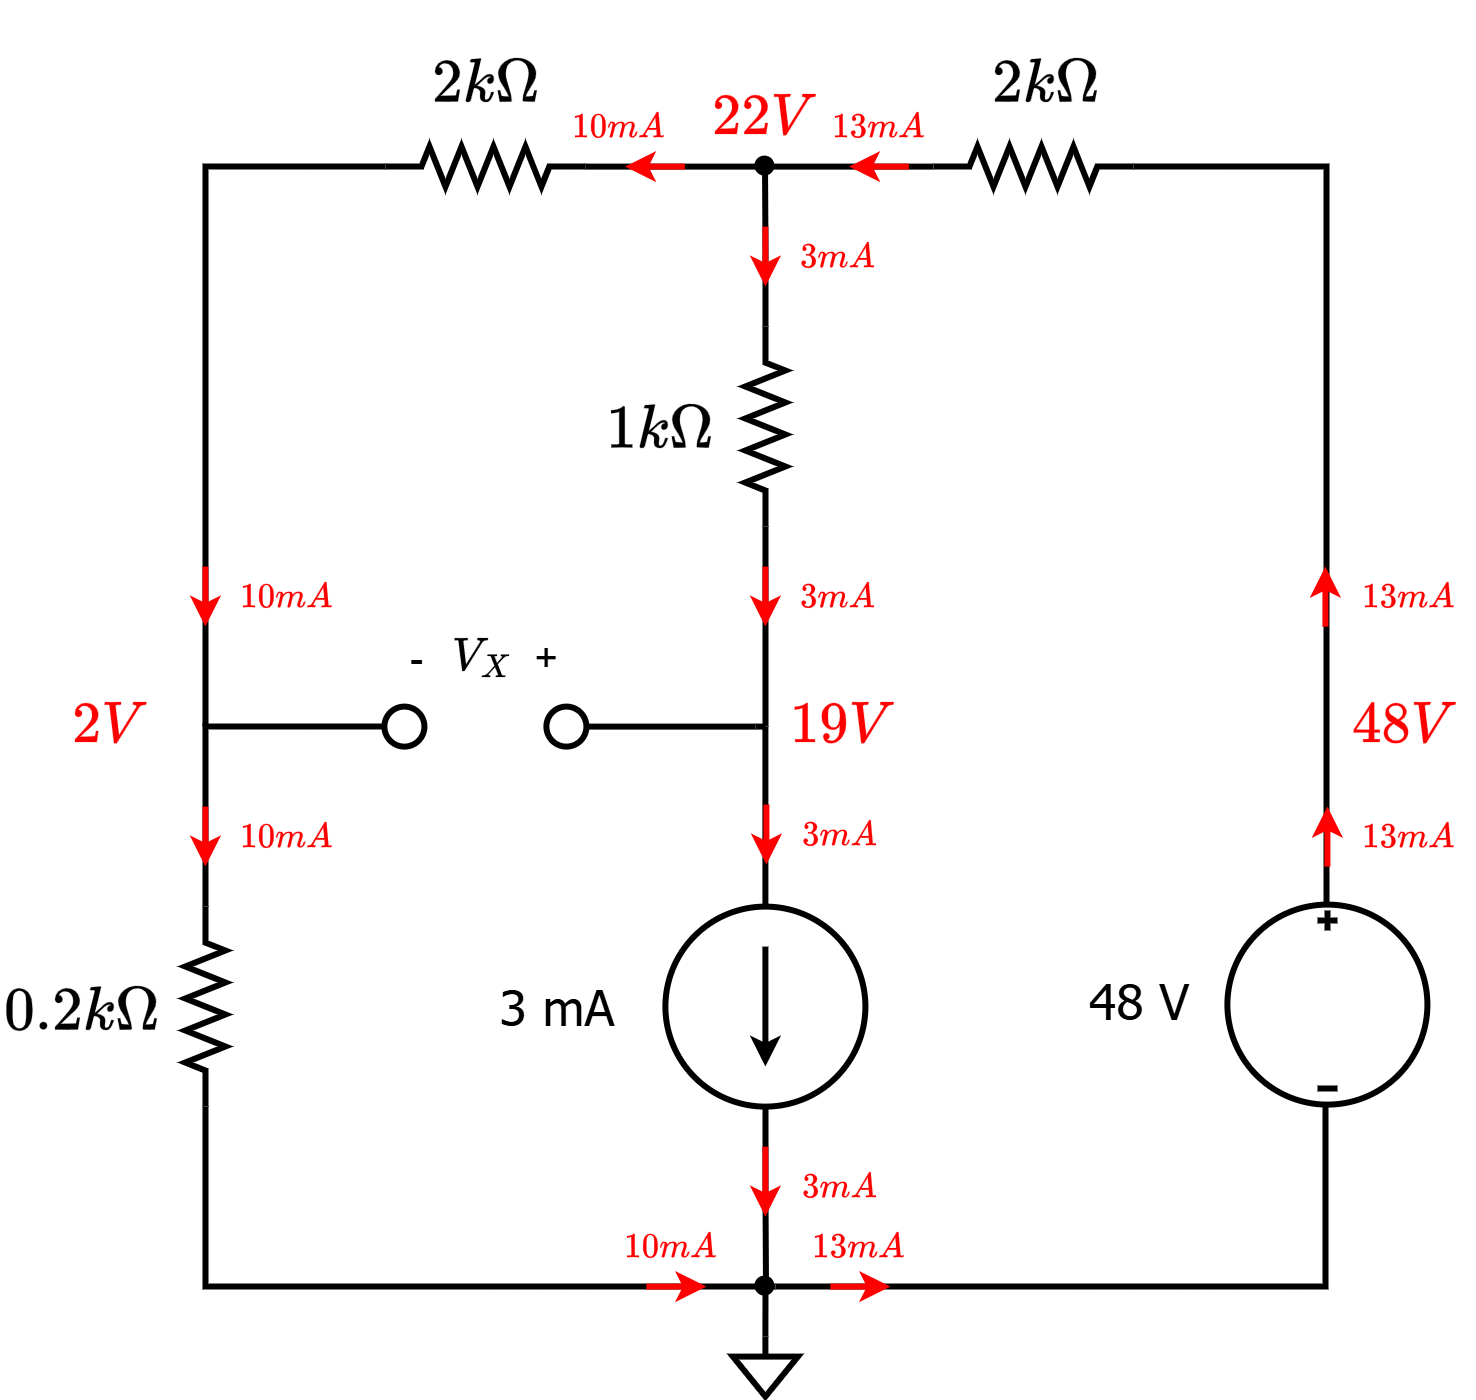
\includegraphics[width=0.5\textwidth]{questionbank/networks/wye_delta_nodal_no_dependent_source/v0/wye_kcl_sol.png}
\end{center}

Subbing in the voltages that we have already found, the problem proceeds just like part (\cref{prob:wye_delta_nodal_no_dependent_source:deltakcl}) for finding the current through the new resistors. Beautifully, the numbers are all familiar and the solution is undisturbed.

We show that KCL is satisfied for all the nodes again. Most nodes now only have two connections so they are quite simple.

At Common: \(13 -3-10  = 0\)

At Node 1: \(10 - 10 = 0\)

At Node 2: \(3-3=0\)

At Node 3: \(13 - 13 = 0\)

At Ground: \(10 + 3-13 = 0\)


Excellent. Consider for a moment how you might have solved the problem if you hadn’t used a Delta-Wye transform.
\end{answer}
\end{partquestion}

\end{mainquestion}

% Problem 5 - Residential Power Distribution Mesh Analysis (24 points)
\clearpage
\Point{residentialpower}{load_estimate}{2}
\Point{residentialpower}{meshanalysis}{12}
\Point{residentialpower}{openneutral}{10}
\Point{residentialpower}{deviceimpact}{2}
\begin{mainquestion}{residentialpower}{Mesh Analysis}
The DC equivalent circuit of a simple residential power distribution is shown below. $R_{w}$ represents the hot wire (typically black) resistance, and $R_{n}$ represents the neutral wire (typically white) resistance. The other resistances represent loads that are drawing power.

\begin{center}
    \includegraphics[width=4in]{../v0/circuit.png}
\end{center}

\begin{partquestion}{load_estimate}
{$R_{1}$ models a heavy duty \qty{2.88}{\kilo\watt} microwave built to run on 120V. \\ $R_{2}$ models a \qty{1.2}{\kilo\watt} blender that draws 10A when crunching ice. \\ $R_{3}$ models a 240V stovetop that draws $\approx\qty{18.5}{\ampere}$ with two of its burners on. \\
Find $R_1$, $R_2$ and $R_3$ to the nearest ohm.}

\begin{answer}
    We can use Ohm's law and the definition of power to find the resistance for each load.
    \[P = \frac{V^2}{R_1} \hspace{1cm} R_1=\frac{120^2}{2880}=5\Omega\]
    \[P = I^2R_2 \hspace{1cm} R_2=\frac{1200}{10^2}=12\Omega\]
    \[R_3 = \frac{V}{I}=\frac{240}{18.5}=13\Omega\]
\end{answer}
\end{partquestion}

\begin{partquestion}{meshanalysis}{Using your results from part (\cref{prob:residentialpower:load_estimate}), use mesh analysis to determine the voltage across each of the three loads given $R_{w}=R_{n}=0.2~\Omega$.}
\begin{answer}
Create three mesh loops in the clockwise direction for the three currents $i_{1}$ in the top-left loop, $i_{2}$ in the bottom-left loop, and $i_{3}$ in the right-hand loop. Using KVL around each loop gives:

\begin{gather*}
R_w i_1 + R_1 (i_1 - i_3) + R_n (i_1 - i_2) = 120 \\
R_w i_2 + R_2 (i_2 - i_3) + R_n (i_2 - i_1) = 120 \\
R_3 i_3 + R_1 (i_3 - i_1) + R_2 (i_3 - i_2) = 0
\end{gather*}

Then we gather like terms:

\begin{gather*}
(R_w + R_1 + R_n)i_1 - R_n i_2 - R_1 i_3 = 120 \\
- R_n i_1 + (R_w + R_2 + R_n)i_2 - R_2 i_3 = 120 \\
- R_1 i_1 - R_2 i_2 + (R_1 + R_2 + R_3)i_3 = 0
\end{gather*}

And this can be neatly written as a matrix:

\[
\begin{bmatrix}
R_w + R_1 + R_n & -R_n & -R_1 \\
-R_n & R_w + R_2 + R_n & -R_2 \\
-R_1 & -R_2 & R_3 + R_1 + R_2
\end{bmatrix}
\begin{bmatrix}
i_1 \\
i_2 \\
i_3
\end{bmatrix}
=
\begin{bmatrix}
120 \\
120 \\
0
\end{bmatrix}
\]

Substituting the given values produces:

\[
\begin{bmatrix}
5.4 & -0.2 & -5 \\
-0.2 & 12.4 & -12 \\
-5 & -12 & 30
\end{bmatrix}
\begin{bmatrix}
i_1 \\
i_2 \\
i_3
\end{bmatrix}
=
\begin{bmatrix}
120 \\
120 \\
0
\end{bmatrix}
\]

This can be solved quickly in MATLAB using matrix inversion, or you can solve by hand. Multiply the second equation by 25 and subtract from the third equation to give:
\[-322i_2+330i_3=-3000\]
Multiply the second equation by 27 and add to the first equation to give:
\[334.6i_2-329i_3=3360\]
From these last two equations, we can eliminate $i_3$ by multiplying the first by 329 and the second by 330 and adding the results.  We get:
\[4480i_2 = 121800\]\[i_2 = \frac{435}{16}\unit{\ampere}\]
	  
Plugging this result back into either previous equation gives \[i_3=\frac{279}{16}\unit{\ampere}\] We can then solve for the first loop current using any of the three original equations, and it is calculated that \[i_1=\frac{315}{8}\unit{\ampere}\] 
In summary:
\begin{align*}
    i_1 &= \frac{315}{8} \approx \qty{39.4}{\ampere}\\
    i_2 &= \frac{435}{16} \approx \qty{27.2}{\ampere}\\
    i_3 &= \frac{279}{16} \approx \qty{17.4}{\ampere}
\end{align*}

The voltages across the three loads are then:
\begin{align*}
v_{1} &= (i_{1}-i_{3}) R_{1} = \left( \frac{315}{8} - \frac{279}{16} \right) 5 = \frac{1755}{16} \approx 109.7~\text{V} \\
v_{2} &= (i_{2}-i_{3}) R_{2} = \left( \frac{435}{16} - \frac{279}{16} \right) 12 = 117~\text{V} \\
v_{3} &= i_{3} R_{3} = \frac{279}{16} \cdot 13 = \frac{3627}{16} \approx 226.7~\text{V}
\end{align*}
\end{answer}
\end{partquestion}

\begin{partquestion}{openneutral}{If a wiring fault occurs such that the neutral becomes an open circuit, recalculate the voltages across the loads.}
\begin{answer}
With the neutral open, $R_{n}\to\infty$ and the left-hand and right-hand loops remain. Let $i_{1}$ be the clockwise current in the left loop and $i_{2}$ be the clockwise current in the right loop.

The KVL system becomes:
\begin{gather*}
R_wi_1 + (R_1 + R_2)(i_1 - i_2) + R_wi_1 = 240 \\
(R_1 + R_2)(i_2 - i_1) + R_3i_2 = 0
\end{gather*}

Gather like terms:
\begin{gather*}
(2R_w + R_1 + R_2)i_1 - (R_1 + R_2)i_2 = 240 \\
- (R_1 + R_2)i_1 + (R_1 + R_2 + R_3)i_2 = 0
\end{gather*}

As a matrix:
\[
\begin{bmatrix}
2R_w + R_1 + R_2 & -R_1 -R_2\\
-R_1 -R_2 & R_1 + R_2 + R_3
\end{bmatrix}
\begin{bmatrix}
i_1 \\
i_2
\end{bmatrix}
=
\begin{bmatrix}
240 \\
0
\end{bmatrix}
\]

Substituting values yields:
\[
\begin{bmatrix}
17.4 & -17\\
-17 & 30
\end{bmatrix}
\begin{bmatrix}
i_1 \\
i_2
\end{bmatrix}
=
\begin{bmatrix}
240 \\
0
\end{bmatrix}
\]

Solving gives $i_{2} = \frac{4080}{233} \approx 17.51~\text{A}$ and $i_{1} = \frac{7200}{233} \approx 30.90~\text{A}$. The load voltages are:
\begin{align*}
v_{1} &= (i_{1}-i_{2})R_1 = \frac{15600}{233} \approx 66.95~\text{V} \\
v_{2} &= (i_{1}-i_{2})R_2 = \frac{13337}{83} \approx 160.7~\text{V} \\
v_{3} &= i_{2} R_3 = \frac{19577}{86} \approx 227.6~\text{V}
\end{align*}
\end{answer}
\end{partquestion}

\begin{partquestion}{deviceimpact}{Suppose $R_2$ now represents a sensitive device. Postulate what might happen to it if it is plugged into this faulty circuit.}
\begin{answer}
Because $R_{2}$ now sees over 160 V instead of the expected 120 V, a sensitive device is likely to be exposed to an overvoltage condition. This can damage components, cause device failure, or lead to unsafe operation.
\end{answer}
\end{partquestion}

\end{mainquestion}

